\section{Passwörter}
\begin{frame}{Passwörter}
  \visible<+->{Wer hat mindestens fünf Online-Accounts?}

  \visible<+->{Wer hat dafür mindestens drei verschiedene Passwörter?}

  \visible<+->{Wer beachtet, Passwörter nur über HTTPS einzugeben?}
\end{frame}

\begin{frame}{Anzahl Passwörter}
  \begin{itemize}
    \item Täglich: Zugangsdaten bei Hackerangriff gestohlen
    \begin{itemize}
      \item Angreifer probieren Zugangsdaten auch anderswo
      \item Schaden lässt sich begrenzen, indem Benutzername und Passwort nirgendwo anders passen
    \end{itemize}
    \item Besonders wichtig: E-Mail-Accounts
    \begin{itemize}
      \item Weil ,,Passwort zurücksetzen`` oft via E-Mail
      \item Wer den E-Mail Account übernommen hat,\\ kann dadurch sämtliche Accounts übernehmen
    \end{itemize}
    \item Ideal: Für jeden Anbieter anderes Passwort
    \item Alternative: Passwörter ,,salzen``
    \begin{itemize}
      \item \textit{passwort}.amz für Onlineshop a
      \item \textit{passwort}.zal für Onlineshop z
      \item \textit{anderespasswort} für Mails
    \end{itemize}
  \end{itemize}
\end{frame}

\begin{frame}{Passwort Wiederverwertung}
  \begin{center}
    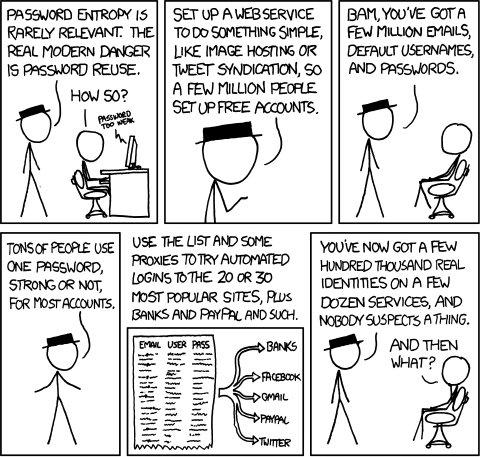
\includegraphics[height=0.8\textheight]{images/password_reuse_top.png}\\
  \end{center}
  \tiny Bildquelle: Ausschnitt aus \href{http://xkcd.com/792/}{xkcd: Password Reuse / CC BY-NC 2.5}
\end{frame}

\begin{frame}{Sichere Passwörter}
  \begin{block}{Anforderungen}
  \begin{itemize}
    \item Klein- und Großbuchstaben, Zahlen,\\ begrenzt: Sonderzeichen
    \item Wichtiger: Lang genug!
  \end{itemize}
  \end{block}
  \begin{block}{Merkbarkeit}
  \begin{itemize}
    \item Pass\emph{satz} statt Passwort\\
      Beispiel: \texttt{margaretthatcheris110\%SEXY}\\
      {\scriptsize (aus Snowden-Interview: \url{https://www.youtube.com/watch?v=yzGzB-yYKcc})}
    \item würfeln, dann sieben zufällige Wörter verwenden\\
      {\scriptsize siehe \url{https://theintercept.com/2015/03/26/passphrases-can-memorize-attackers-cant-guess/}}
  \end{itemize}
  \end{block}
\end{frame}

\begin{frame}{Passwort Länge vs. Zeichensatz}
  \begin{center}
    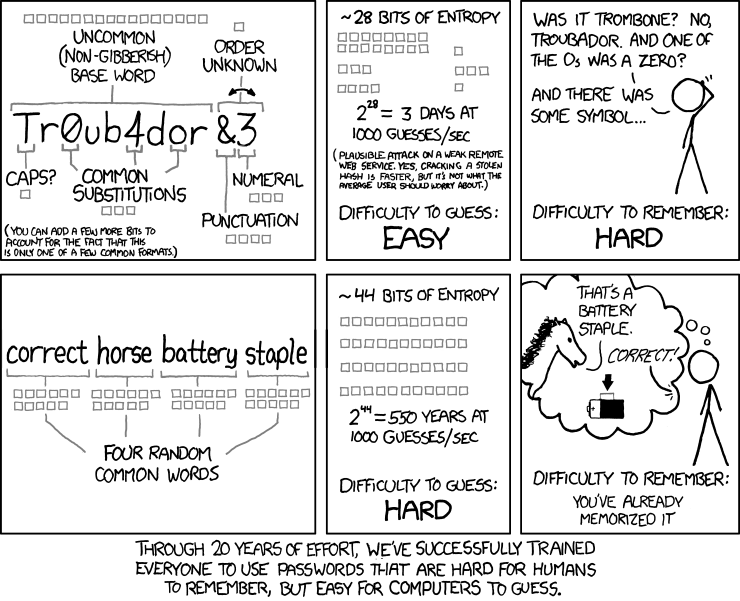
\includegraphics[width=0.99\textheight]{images/password_strength.png}\\
  \end{center}
  \tiny Bildquelle: \href{http://xkcd.com/936/}{xkcd: Password Strength / CC BY-NC 2.5}
\end{frame}

\begin{frame}{Passwort-Manager}
  \begin{itemize}
    \item Verwalten Passwörter in verschlüsselter Datenbank
    \item Anwender muss sich nur noch \emph{ein} Passwort merken
  \end{itemize}
  \pause
  \begin{columns}[T]
    \begin{column}{.48\textwidth}
      \small
      \begin{blit}{Vorteile}
        \item Erzeugt echt zufällige Passwörter
        \item Erleichtert\\ für jeden Anbieter\\ anderes Passwort
      \end{blit}
    \end{column}
    \begin{column}{.48\textwidth}
      \small
      \begin{blit}{Nachteile}
        \item Eingefangene Malware\\bekommt alle Passwörter\\auf einmal
      \end{blit}
    \end{column}
  \end{columns}
  \pause
  \begin{blit}{Anmerkungen}
    \item Bei lokalen Datenbanken: Datei+Passwort (2 Dinge)
    \item Bei online Datenbanken: Nur Passwort (Bruteforce!)
    \item Backups machen \& wichtige Passwörter merken!\\ (Computer defekt, gestohlen)
    \item Unsere Empfehlung: KeePass(X)
  \end{blit}
\end{frame}

\endinput
